\iffalse
\let\negmedspace\undefined
\let\negthickspace\undefined
\documentclass[journal,12pt,twocolumn]{IEEEtran}
\usepackage{cite}
\usepackage{amsmath,amssymb,amsfonts,amsthm}
\usepackage{algorithmic}
\usepackage{graphicx}
\usepackage{textcomp}
\usepackage{xcolor}
\usepackage{txfonts}
\usepackage{listings}
\usepackage{enumitem}
\usepackage{mathtools}
\usepackage{gensymb}
\usepackage{comment}
\usepackage[breaklinks=true]{hyperref}
\usepackage{tkz-euclide} 
\usepackage{listings}
\usepackage{gvv}                                    
\usepackage{tikz}
\usepackage{pgfplots}
\def\inputGnumericTable{}                                 
\usepackage[latin1]{inputenc}                                
\usepackage{color}                                            
\usepackage{array}                                            
\usepackage{longtable}                                       
\usepackage{calc}                                             
\usepackage{multirow}                                         
\usepackage{hhline}                                           
\usepackage{ifthen}                                           
\usepackage{lscape}
\usepackage{circuitikz}
\newtheorem{theorem}{Theorem}[section]
\newtheorem{problem}{Problem}
\newtheorem{proposition}{Proposition}[section]
\newtheorem{lemma}{Lemma}[section]
\newtheorem{corollary}[theorem]{Corollary}
\newtheorem{example}{Example}[section]
\newtheorem{definition}[problem]{Definition}
\newcommand{\BEQA}{\begin{eqnarray}}
\newcommand{\EEQA}{\end{eqnarray}}
\newcommand{\define}{\stackrel{\triangle}{=}}
\theoremstyle{remark}
\newtheorem{rem}{Remark}
\usetikzlibrary{positioning, arrows.meta}
\begin{document}
% Define custom function M(f)
\pgfmathdeclarefunction{Mf}{1}{%
  \pgfmathparse{sin(deg(#1))}%
}

\parindent 0px
\bibliographystyle{IEEEtran}

\title{GATE - BM 22}
\author{EE23BTECH11215 - Penmetsa Srikar Varma$^{}$% <-this % stops a space
}
\maketitle
\newpage
\bigskip

\renewcommand{\thefigure}{\theenumi}
\renewcommand{\thetable}{\theenumi}
\section*{Question}
A continous time transfer function, $\text{H\brak{\text{s}}}=\frac{1+\frac{\text{s}}{10^6}}{\text{s}}$ is coverted to a discrete time transfer function, $\text{H\brak{\text{z}}}$ using a bi-linear transformation at 100 MHz sampling rate. The pole of $\text{H\brak{\text{z}}}$ is located at z = ?\hfill \brak{\text{GATE BM 2021}}
\section*{Solution}
\fi
\begin{table}[h]
    \centering
    \begin{tabular}{|c|c|}
    \hline
        Variable & Condition \\
    \hline
         $\text{F}_\text{s}$ = 100 MHz & sampling rate \\
    \hline
         $\text{T}_\text{s}$ = $\frac{1}{\text{F}_\text{s}}$ & sampling period \\
    \hline
       $\text{s}_0$ & pole of $\text{H\brak{\text{z}}}$ \\
    \hline
\end{tabular}

    \label{parameter table}
\end{table}
\begin{center}
    Table of Parameters
\end{center}

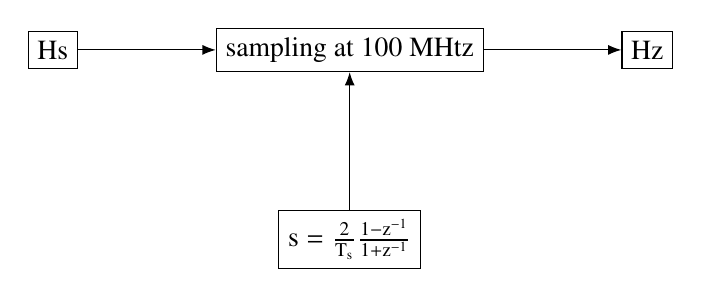
\begin{tikzpicture}[auto, node distance=1.75cm,>=Latex]
    % Define blocks
    \node [draw, rectangle] (input) {\(\text{H\brak{\text{s}}}\)};
    \node [draw, rectangle, right=of input] (system) {sampling $\brak{\text{at 100 MHtz}}$ };
    \node [draw, rectangle, right=of system] (output) {\(\text{H\brak{\text{z}}}\)};
    \node [draw, rectangle, below=of system] (default) {$\text{s}=\frac{2}{\text{T}_\text{s}}\brak{\frac{1-\text{z}^{-1}}{1+\text{z}^{-1}}}$};
    
    % Connect blocks
    \draw [->] (input) -- (system);
    \draw [->] (system) -- (output);
    \draw [->] (default) -- (system);
\end{tikzpicture}\\

From above,
\begin{align}
\label{gate,2k21,bm22,eq}
    \text{H\brak{\text{z}}}&=\text{H}\brak{2\text{F}_\text{s}\brak{\frac{1-\text{z}^{-1}}{1+\text{z}^{-1}}}}
\end{align}
So, from \brak{\ref{gate,2k21,bm22,eq}}
\begin{align}
    \text{H\brak{\text{z}}}&=\frac{1+\frac{2\text{F}_{\text{s}}}{10^6}\brak{\frac{1-\text{z}^{-1}}{1+\text{z}^{-1}}}}{2\text{F}_{\text{s}}\brak{\frac{1-\text{z}^{-1}}{1+\text{z}^{-1}}}}
\end{align}
\begin{align}
    \text{H\brak{\text{z}}}&=\frac{1}{200\times10^6}\brak{\frac{1+\text{z}^{-1}+200\brak{1-z^{-1}}}{1-z^{-1}}}
\end{align}
\begin{align}
    \text{H\brak{\text{z}}}&=5\times10^{-9}\brak{\frac{201-199\text{z}^{-1}}{1-z^{-1}}}
\end{align}
So, $\text{s}_0$ is at z=1\\

%\end{document}
